\mychapter{Resultados e Discussões}{cap:resultados}    

Apresentamos o desenvolvimento de uma ferramenta portável, rápida e de boa qualidade numérica que possibilita gerar novos métodos de interação do usuário com o sistema de análise, permitindo que este seja capaz de analisar os diferentes descritores oriundos da Teoria da Informação e permitir a análise gráfica dos resultados.

Seguindo o modelo de engenharia de software em espiral, o sistema foi projetado e desenvolvido de forma modular, composto pelas seguintes unidades:

\begin{itemize}
\item Módulo de simbolização;
\item Módulo de análise;
\item Modulo de visualização e interação (Em fase de desenvolvimento);
\end{itemize} 

Esses módulos foram e estão sendo desenvolvidos seguindo um cronograma. 
Depois passaram pelas seguintes etapas:

\begin{itemize}
\item Integração dos módulos em um sistema;
\item Teste e validação do sistema;
\item Geração da interface gráfica.
\end{itemize}

Permite-se a leitura de dados em vários formatos (TXT, CSV ou XLSX), e o usuário a seguir poderá escolher:

\begin{itemize}

	\item Gerar o gráfico da série (ver Figura 1);
	\item Calcular seus diversos valores de Entropia;
	\item Calcular seus diversos valores de Distâncias Estocásticas;
	\item Calcular complexidades estatísticas;
    \item Identificar padrões no gráfico da série temporal;
    \item Gerar planos de Entropias;
    \item Gerar planos de Distâncias Estocásticas;
	\item Gerar o histograma de padrões (ver Figura 1);
	\item Identificar o ponto característico da série no plano Entropia-Complexidade (ver Figura 1).

\end{itemize}

Um elemento original do sistema é a vinculação entre o histograma de padrões, formado através do processo de simbolização de Bandt-Pompe ~\citep{Bandt2002Permutation}, e a série temporal. 
Escolhendo um ou mais elementos do histograma, os valores correspondentes na série temporal aparecem realçados. 
Esta funcionalidade permite a análise visual da distribuição temporal dos padrões, possibilitando futuramente a realização de outros testes.
 
O teste e a validação do sistema foram tarefas contínuas ao longo do desenvolvimento do projeto, bem como o incremento do desenvolvimento de novas funcionalidades. 

Com a troca da ferramenta de interface, foi necessário primeiramente um estudo de documentações referentes ao pacote gráfico~\citep{rgtk2}. 
Uma vez que ocorreu uma mudança de paradigmas, pois a biblioteca escolhida funciona por meio de blocos verticais e horizontais, onde os horizontais se são distribuídos diante dos verticais, foram encontrados os seguintes problemas durante a implementação:

\begin{itemize}
\item A reprodução do modelo do protótipo;
\item A implementação da função referente a \texttt file.choose em \texttt R, pois o escopo das variáveis declaradas dentro das funções de tratamento de interrupções é local;
\item A implementação das funções de tratamento de interrupção;
\item O desenvolvimento da parte estética do software.
\end{itemize}

\begin{figure}
  \centering
  \caption{Estrutura de organização dos componentes no RGtk2}
   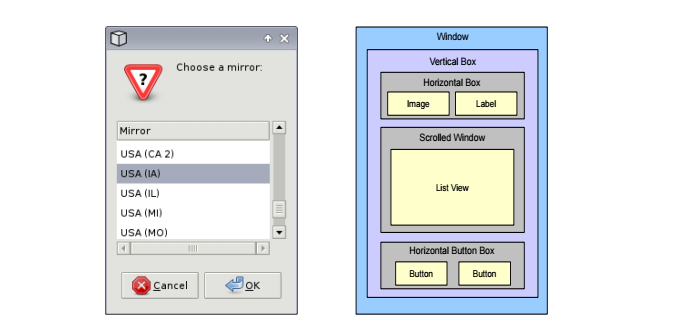
\includegraphics[width=10cm,height=6cm]{capitulos/imagens/rgtk2.png}
\end{figure}
  
\begin{figure}[H]
	\centering
	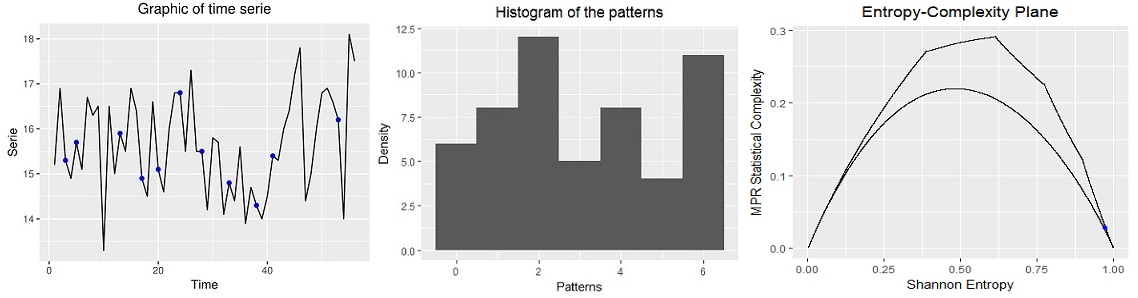
\includegraphics[width=1\columnwidth]{capitulos/imagens/rplot}        
    \caption{Representação gráfica da análise de uma série temporal de produção anual de cevada por acre.}
\end{figure}
 
\begin{figure}[H]
	\centering
	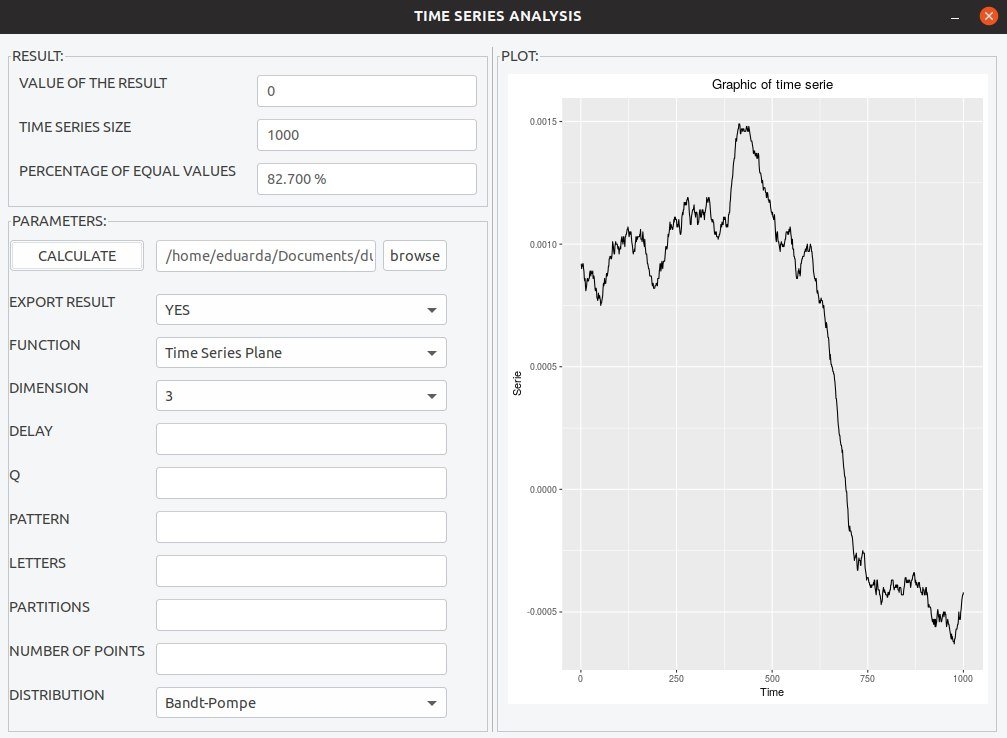
\includegraphics[width=0.95\columnwidth]{capitulos/imagens/SoftwareNow.jpg}   
    \caption{Imagem atual do software.}
    \vspace{6cm}
\end{figure}


